
\pdfoutput=1
\pdfpagewidth=8.5in
\pdfpageheight=11in
\documentclass[10pt,conference]{IEEEtran}

\usepackage[T1]{fontenc}
\usepackage[utf8]{inputenc}
\usepackage{microtype}
\usepackage{cite}
\usepackage{graphicx}
\usepackage{booktabs}
\usepackage{amsmath,amssymb,amsthm}
\usepackage{algorithm}
\usepackage{algpseudocode}
\usepackage{tikz}
\usetikzlibrary{arrows.meta,positioning,shapes.geometric}
\usepackage{xspace}

\newcommand{\PopulationSize}{1445}
\newcommand{\MeanVoilaAccuracy}{70.5}
\newcommand{\MeanVoilaMB}{0.136}
\newcommand{\MeanFullAccuracy}{63.2}
\newcommand{\MeanFullMB}{5.521}
\newcommand{\MeanByteReduction}{97.5}
\newcommand{\OneSecondVoilaDQA}{70.3}
\newcommand{\OneSecondFullDQA}{37.9}
\newcommand{\CpuPFiftyMs}{4.12}

\DeclareMathOperator*{\argmax}{arg\,max}
\newcommand{\system}{\textsc{VOILA}\xspace}
\newcommand{\fset}{\mathcal{F}}
\newcommand{\bytes}{\operatorname{bytes}}
\newcommand{\dqa}{\operatorname{DQA}}
\newcommand{\tableformat}{\footnotesize\setlength{\tabcolsep}{3.5pt}\renewcommand{\arraystretch}{0.95}}
\newtheorem{proposition}{Proposition}

\title{VOILA: Value-of-Information Guided Visual Fidelity Selection for Bandwidth-Constrained settings}
\author{\IEEEauthorblockN{Anonymous Authors}}

\begin{document}
\maketitle

\begin{abstract}
Visual evidence is commonly acquired at a fixed fidelity even when the query
does not require all of its detail. This design pays the transmission or
retrieval cost before a remote vision--language model (VLM) can decide whether
that detail was useful. We study \emph{pre-retrieval fidelity selection}: given
the question and cached metadata, choose which visual representation to acquire
before accessing its pixels or invoking the VLM. The central hypothesis is
that linguistic structure predicts visual information need. \system learns a
success predictor for each fidelity, calibrates the predictors independently,
and selects the representation maximizing predicted correctness minus its
measured byte cost. We evaluate six VLMs on the same \PopulationSize-query
FloodNet population using five image-grouped folds with disjoint training,
calibration, operating-point validation, and test images. \system obtains
\MeanVoilaAccuracy\% mean accuracy at \MeanVoilaMB\ MB/query, reducing bytes by
\MeanByteReduction\% relative to transmitting full images. Against the best
fixed fidelity, it matches one-second deadline-qualified accuracy while reducing
mean payload by roughly 62\%, with a 0.6--1.7 point accuracy cost on four models
and accuracy gains on LLaVA and Pixtral. The benefit is not universal: a strong
fixed thumbnail policy is best for Qwen2-VL-72B, and unseen question templates
reduce accuracy by 17.4--37.1 points. These results show when language can guide
information acquisition before transmission, and expose calibration, model
preprocessing, and linguistic shift as the principal constraints.
\end{abstract}

\section{Introduction}
\label{sec:introduction}

Multimodal systems increasingly separate where visual data is captured from
where it is interpreted. Images may be retained as captions, thumbnails,
compressed previews, and full-resolution originals, while an expensive VLM is
invoked remotely~\cite{alayrac2022flamingo,li2023blip2,liu2024visual,bai2023qwen}.
The usual pipeline acquires the highest-fidelity representation first and asks
whether it was necessary afterward. This order hides an important decision:
\emph{what evidence should be retrieved or transmitted before inference?}

Flood response provides a concrete instance. Aerial capture can produce images
faster than a disrupted or congested uplink can deliver them, while analysts
ask questions such as \emph{``What is the overall condition of this area?''}
and \emph{``How many buildings are flooded?''}~\cite{rahnemoonfar2021floodnet}.
The former often depends on coarse scene semantics; the latter depends on
small-object detail. Sending every original preserves the possibility of
answering either question, but consumes the scarce link before the question's
information need is considered. Sending every thumbnail saves bytes but can
destroy the evidence required by counting and localization.

This motivates a pre-retrieval, or equivalently pre-transmission, stage that is
orthogonal to model routing. Model cascades and early-exit methods reduce the
computation applied after context is available~\cite{chen2023frugalgpt,
ding2024hybrid,wang2024routellm,zhou2020bert,schuster2022confident}.
Compression, adaptive video analytics, edge offloading, semantic
communication, and visual-token reduction reduce representation or compute
after inspecting data or executing part of the pipeline~\cite{
toderici2016variablerateimagecompression,weng2024learning,
jiang2018chameleon,du2020dds,li2020reducto,kang2017neurosurgeon,
xie2021semantic,cai2024matryoshka,chen2024fastv}. Neither
answers which cached representation should cross the storage or network
boundary in the first place.

The core question is therefore: \textbf{can the language of a question predict
the visual fidelity that a remote VLM will need?} Two questions over the same
asset can express very different evidence requirements. Phrases such as
\emph{how many} imply enumeration of small instances, whereas \emph{overall
condition} asks for scene-level recognition. Prior work shows that question
form predicts VQA difficulty~\cite{kafle2017analysis,agrawal2018dont} and that
query features can predict retrieval quality before retrieval~\cite{
zhao2008predicting,hauff2008improved,mothe2005linguistic}. We investigate
whether this signal is strong enough to select visual fidelity under an actual
byte budget.

The decision is harder than ordinary classification. Correctness is
non-monotone in fidelity for modern VLMs; a compressed representation can
outperform an original by suppressing irrelevant detail. Raw success scores
cannot be compared as probabilities across fidelities, and VLM log
probabilities are available only after paying the acquisition and inference
cost. A useful policy must estimate counterfactual success before image access,
calibrate those estimates on disjoint data, and attach them to the measured
size of each cached representation.

We introduce \system, a language-conditioned, value-of-information policy for
this stage. For every candidate fidelity, a lightweight predictor estimates
whether the target VLM would answer correctly. An independent isotonic map
turns each score into a probability, and a validation-selected byte penalty
chooses the representation with the largest predicted correctness minus exact
payload cost. The selected representation is acquired once and the remote VLM
is invoked once.

This paper makes four contributions:
\begin{itemize}
  \item We formulate pre-retrieval visual fidelity selection as cost-sensitive
  information acquisition, distinct from post-retrieval model routing.
  \item We show on FloodNet that question form predicts fidelity need, while no
  fixed fidelity is uniformly best across six VLMs.
  \item We develop a leakage-resistant calibrated selection pipeline and a
  validation-only operating-point rule using measured, item-specific bytes.
  \item We evaluate accuracy--byte frontiers, matched-policy comparisons,
  mission budgets, and deadline-qualified accuracy using six public cellular
  scenarios, while reporting the cases in which fixed or supervised routing
  remains stronger.
\end{itemize}

\section{Motivating Observation}
\label{sec:observation}

\begin{figure*}[t]
  \centering
  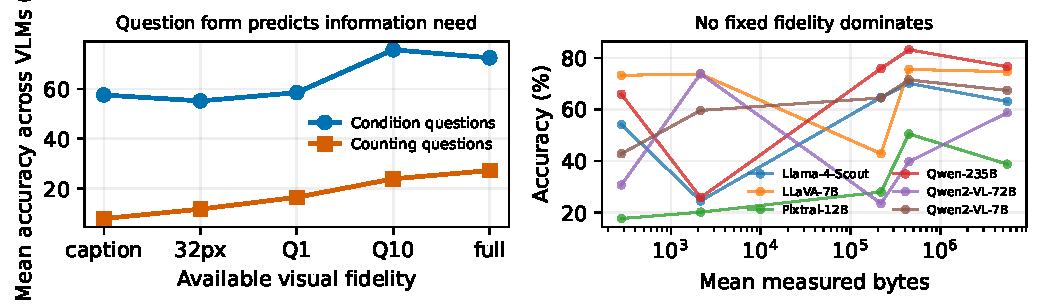
\includegraphics[width=0.94\textwidth]{generated/motivating_observation.pdf}
  \caption{The motivating observation on the common FloodNet population.
  Left: mean VLM accuracy separated only by the linguistic form of the
  question; counting benefits most from detail, while condition recognition
  peaks at a compressed fidelity. Right: fixed-fidelity curves differ sharply
  across the six VLMs, so neither full resolution nor one compressed tier is a
  universal choice. Values are computed from cached answers on the same
  image-grouped population used in the main evaluation.}
  \label{fig:motivation}
\end{figure*}

\textbf{Question form separates visual information requirements.}
Figure~\ref{fig:motivation} (left) groups FloodNet questions using only their
surface form. Across all six VLMs, questions beginning with \emph{how many}
gain as more visual detail becomes available. Condition-recognition questions
instead peak at JPEG Q10 on average and frequently succeed from a cached
caption or thumbnail. This is not a claim that language determines the answer;
it predicts how much visual evidence is likely to be useful before that
evidence is acquired.

\textbf{More pixels do not imply a better answer.}
Figure~\ref{fig:motivation} (right) shows the five fixed-fidelity curves. Their
non-monotonicity is substantial: LLaVA is strong on captions and 32-pixel
images, Qwen2-VL-72B peaks at 32 pixels, and Pixtral benefits from JPEG Q10.
Full resolution is not the most accurate fixed input for any evaluated model.
The selection problem is therefore not reducible to estimating the smallest
image that approximates the original; it must estimate VLM success directly.

\textbf{Post-hoc confidence arrives too late and can be misleading.}
A cascade must first retrieve a representation, run the VLM, and then inspect
its confidence. When visual grounding is weak, fluent answers driven by
language priors can still receive high probability. This is precisely the
failure mode observed for the cumulative-cost Log-prob Cascade in
Section~\ref{sec:results}: confidence-based escalation is both post-retrieval
and poorly aligned with missing visual information. These observations motivate
a language-only predictor whose scores are explicitly calibrated for comparing
fidelities.

\begin{table}[t]
\centering
\tableformat
\caption{Fixed-fidelity accuracy (\%) underlying
Figure~\ref{fig:motivation}. The best input is model-dependent and is never the
full image in this population.}
\label{tab:fixed}
\begin{tabular}{lrrrrr}
\toprule
Model & Caption & 32px & Q1 & Q10 & Full \\
\midrule
Llama-4-Scout & 54.2 & 24.6 & 64.7 & 70.2 & 63.1 \\
LLaVA-7B & 73.3 & 73.8 & 42.9 & 75.6 & 74.7 \\
Pixtral-12B & 17.7 & 20.2 & 28.0 & 50.5 & 38.8 \\
Qwen-235B & 66.0 & 25.8 & 75.9 & 83.2 & 76.6 \\
Qwen2-VL-72B & 30.7 & 73.9 & 23.6 & 39.8 & 58.8 \\
Qwen2-VL-7B & 42.8 & 59.7 & 64.5 & 71.5 & 67.4 \\
\bottomrule
\end{tabular}

\end{table}

\section{Problem Formulation}
\label{sec:problem}

Let $q$ be a question associated with a visual asset $x$, and let
$\fset=\{f_1,\ldots,f_K\}$ be cached representations ordered by nominal
fidelity. In our implementation these are an offline cached caption generated
once at ingestion, a $32\!\times\!32$ PNG, JPEG Q1, JPEG Q10, and the original
image.
The client can read each representation's stored byte count $b_f(x)$ from
metadata without accessing its content. Let $M$ be a fixed remote VLM and
$Y_f(q,x)\in\{0,1\}$ indicate whether $M$ answers correctly when given $f$.

The pre-retrieval policy does not observe any $Y_f$ at decision time. It must
estimate
\begin{equation}
  p_f(q)=\Pr\!\left[Y_f(q,x)=1\mid \phi(q)\right],
  \label{eq:success}
\end{equation}
where $\phi(q)$ contains only linguistic features. Given a byte price
$\lambda\geq0$, the one-step value-of-information decision is
\begin{equation}
  f^*(q,x)=\argmax_{f\in\fset}
  \left[\widehat p_f(q)-\lambda b_f(x)\right].
  \label{eq:utility}
\end{equation}
This objective treats an expected correct answer as unit utility and charges
the exact bytes that cross the boundary. Other deployments may substitute a
monetary, energy, or latency cost without changing the estimator.

Three properties make Eq.~\ref{eq:utility} difficult. First, its labels are
counterfactual: offline training must evaluate every fidelity, but online
selection is useful only if it avoids doing so. Second, a raw classifier score
for captions is not commensurate with a raw score for full images. Utility
subtraction is meaningful only when each is mapped to a probability on held-out
data~\cite{guo2017calibrationmodernneuralnetworks,desai2020calibration}. Third,
images and repeated question templates create leakage paths. Random row splits
can place nearly identical evidence on both sides of evaluation. We therefore
separate images across all stages and test template shift independently.

Calibration matters because errors are paid twice: an underestimated useful
fidelity can remove answer evidence, while an overestimated one wastes bytes.
The following standard decision-regret argument makes the dependence explicit.

\begin{proposition}[Selection regret under calibrated estimation]
Let $p_f$ be the true conditional success probabilities and suppose
$|\widehat p_f-p_f|\leq\epsilon$ for every $f\in\fset$. If $f^*$ maximizes the
true utility $p_f-\lambda b_f$ and $\widehat f$ maximizes
$\widehat p_f-\lambda b_f$, then
\[
 (p_{f^*}-\lambda b_{f^*})-(p_{\widehat f}-\lambda b_{\widehat f})
 \leq 2\epsilon.
\]
\end{proposition}
\begin{proof}
Add and subtract the two estimated utilities. The middle difference is
non-positive because $\widehat f$ maximizes estimated utility; each remaining
probability error is at most $\epsilon$.
\end{proof}

The result does not assert that isotonic regression always has the smallest
finite-sample error. It states why the system needs probabilities whose errors
are controlled on data separate from both predictor fitting and operating-point
selection. The calibration ablation in Section~\ref{sec:results} tests that
choice rather than assuming it.

\section{System Design}
\label{sec:design}

\begin{figure*}[t]
\centering
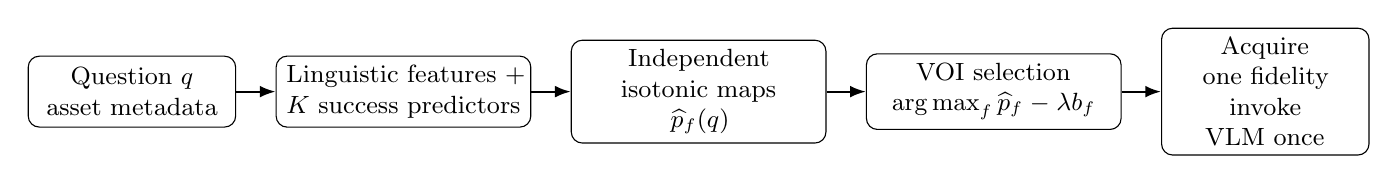
\begin{tikzpicture}[
  font=\small,
  box/.style={draw,rounded corners,align=center,minimum height=9mm,text width=24mm},
  wide/.style={draw,rounded corners,align=center,minimum height=9mm,text width=30mm},
  arrow/.style={-{Latex[length=2mm]},thick},
  node distance=4mm and 5mm]
\node[box] (query) {Question $q$\\asset metadata};
\node[wide,right=of query] (predict) {Linguistic features +\\$K$ success predictors};
\node[wide,right=of predict] (cal) {Independent isotonic maps\\$\widehat p_f(q)$};
\node[wide,right=of cal] (select) {VOI selection\\$\argmax_f\widehat p_f-\lambda b_f$};
\node[box,right=of select] (send) {Acquire one fidelity\\invoke VLM once};
\draw[arrow] (query)--(predict);
\draw[arrow] (predict)--(cal);
\draw[arrow] (cal)--(select);
\draw[arrow] (select)--(send);
\end{tikzpicture}
\caption{\system deployment topology. An edge client or gateway holds a compact
metadata index over cached cloud/archive representations and chooses one payload
before transmission to the remote VLM. The decision reads the question and byte
metadata, but no pixels. Caption generation occurs once during ingestion; online
accounting includes only the selected cached payload.}
\label{fig:system}
\end{figure*}

\subsection{Offline success learning}

For a target VLM, the offline stage records correctness at every fidelity on
labeled examples. We extract sparse TF--IDF features and structural indicators
for counting, condition, yes/no form, numerals, negation, and question length.
A fidelity-specific gradient-boosted predictor $g_f$ produces a score
$r_f(q)=g_f(\phi(q))$. The predictors model the behavior of the target VLM;
they do not replace it and never consume the visual representation.

The feature representation deliberately separates lexical and structural cues:
TF--IDF captures distinctions between repeated question forms, while
structural features represent properties expected to transfer beyond a single
vocabulary. Examples include an initial \emph{how many}, a yes/no auxiliary,
numeric tokens, negation, and question length. This design tests the linguistic
hypothesis directly and keeps the selection stage independent of a second
large language model. A richer encoder remains a baseline rather than an
unpriced component of \system.

We fit an independent isotonic calibrator $\psi_f$ on a population disjoint
from predictor training:
\begin{equation}
  \widehat p_f(q)=\psi_f(r_f(q)).
  \label{eq:calibration}
\end{equation}
Independent maps are necessary because score scales and error rates differ by
fidelity. Isotonic regression preserves each predictor's rank while learning a
non-parametric mapping to empirical correctness~\cite{
guo2017calibrationmodernneuralnetworks}. It does not impose cross-fidelity
monotonicity, because Figure~\ref{fig:motivation} shows that VLM correctness is
not monotone in pixels.

\subsection{Validation-only operating point}

For each outer fold, a separate validation population selects $\lambda$.
Let $A_{\mathrm{fix}}^{\mathrm{val}}$ be the accuracy of the best fixed
fidelity on validation data. Among candidate penalties whose validation
accuracy is at least $0.95A_{\mathrm{fix}}^{\mathrm{val}}$, we choose the one
with the smallest measured mean bytes. Neither the test answers nor test costs
choose the operating point. This rule yields a deployable point rather than
selecting the most attractive location after seeing the test frontier.

\subsection{Online selection and system boundary}

Algorithm~\ref{alg:voila} summarizes inference. The client reads $q$ and the
already-indexed byte lengths, evaluates the lightweight predictors and
calibrators, and acquires exactly one representation. The remote VLM is then
called once. The boundary excludes one-time caption generation, because
captions are cached during ingestion, and includes the exact selected payload.
The design composes with model routing: after acquisition, another policy may
still choose which remote model processes the evidence.

The intended topology is an edge--cloud or archive--cloud split rather than an
on-drone VLM deployment. A drone, phone, or field gateway has the user's
question and an index containing asset identifiers, byte counts, and cached
caption pointers. The high-volume image tiers reside in remote object storage or
at a nearby gateway. \system runs at the requester or gateway, selects one tier,
and only then transmits that payload to the VLM service. This is why
Figure~\ref{fig:system} is a placement diagram as well as a pipeline: the
decision is made before the expensive network/storage boundary, not between VLM
layers.

\begin{algorithm}[t]
\caption{\system pre-retrieval fidelity selection}
\label{alg:voila}
\begin{algorithmic}[1]
\Require question $q$, asset metadata $\{b_f(x)\}_{f\in\fset}$,
predictors $g_f$, calibrators $\psi_f$, validation-selected $\lambda$
\ForAll{$f\in\fset$}
  \State $r_f\gets g_f(\phi(q))$
  \State $\widehat p_f\gets\psi_f(r_f)$
  \State $u_f\gets\widehat p_f-\lambda b_f(x)$
\EndFor
\State $f^*\gets\argmax_{f\in\fset}u_f$
\State acquire $x$ at $f^*$; invoke the remote VLM once
\State \Return the VLM answer and selected fidelity $f^*$
\end{algorithmic}
\end{algorithm}

The algorithm differs from a sequential cascade in both action and accounting.
It evaluates all $K$ lightweight success predictors, but it does not acquire
$K$ visual inputs and does not invoke the VLM $K$ times. It also allows the
selected fidelity to skip intermediate tiers. This is essential when a caption
and an original are cached independently: the cost of choosing the original is
its payload, not the sum of every lower-quality representation. We retain the
cumulative rule only as a legacy ablation.

\section{Experimental Method}
\label{sec:evaluation}

The evaluation answers three questions. \textbf{RQ1} asks whether linguistic
pre-retrieval selection improves the measured accuracy--byte frontier over
fixed and adaptive policies. \textbf{RQ2} asks whether byte reductions produce
more correct answers under upload deadlines and shared mission budgets.
\textbf{RQ3} asks which calibration and feature choices enable the result, and
where the linguistic assumption fails.

\subsection{Driving use case and population}

We use FloodNet as the driving case because it pairs aerial flood imagery with
questions whose visual requirements range from scene condition to object
counting~\cite{rahnemoonfar2021floodnet}. The common population contains
\PopulationSize{} query records for which all five cached fidelities and all six
VLM outputs are available. The models span LLaVA-7B, Pixtral-12B, Llama-4-Scout,
Qwen2-VL-7B, Qwen2-VL-72B, and Qwen-235B~\cite{zhou2024tinyllava,pixtral2024,
abdullah2025evolutionmetasllamamodels,Qwen2VL,bai2023qwen}. We make no new VLM
or API calls; cached outputs are the only source of answer correctness.

\begin{table}[t]
\centering
\tableformat
\caption{Measured cached representation sizes on the common FloodNet
population. The router reads these byte counts as metadata.}
\label{tab:sizes}
\begin{tabular}{lrrr}
\toprule
Representation & Median & p95 & Mean bytes \\
\midrule
Cached caption & 188 & 663 & 281 \\
32$	imes$32 PNG & 2,125 & 2,605 & 2,141 \\
JPEG Q1 & 213,991 & 248,887 & 217,576 \\
JPEG Q10 & 432,120 & 638,742 & 445,479 \\
Full image & 5,195,608 & 7,622,159 & 5,520,774 \\
\bottomrule
\end{tabular}

\end{table}

Table~\ref{tab:sizes} reports measured bytes rather than a normalized proxy.
Each outer test fold holds out images, not rows. The remaining images are split
again into mutually disjoint predictor-training, calibration, and
operating-point-validation populations. We use five outer folds and report
query-level selections for every policy. Confidence intervals and paired
differences resample image clusters, keeping questions from the same image
together.

This separation is stricter than a conventional train/test split. Predictor
training learns $g_f$; calibration alone fits $\psi_f$; validation alone chooses
$\lambda$ and the best fixed comparator; and the test fold is used once for
reporting. Because the unit of assignment is the image, questions sharing the
same visual evidence cannot cross these boundaries. The leave-template-out
stress test then changes the grouping variable to ask a different question:
whether the learned linguistic regularities survive unseen phrasing.

\subsection{Policies and metrics}

We compare all five fixed fidelities; the cross-validated best fixed fidelity;
a cumulative-cost Log-prob Cascade inspired by FrugalGPT~\cite{
chen2023frugalgpt}; a supervised BERT Router; the earlier sequential \system
rule as an ablation; and a cached hindsight oracle. The GPT-4o router is omitted
because its cached labels do not cover the complete common population. The
primary metrics are correctness, exact transmitted bytes, bytes at matched
accuracy, and accuracy at matched cost.

For network consequences, we simulate one-way evidence serialization using six
public CellReplay scenarios~\cite{cellreplay-nsdi25}: T-Mobile driving,
stationary-good, and weak-signal; and Verizon crowded, stationary-good, and
walking. The simulator consumes the recorded \texttt{up-heavy-pdo},
\texttt{up-delay-light-pdo}, and \texttt{latency-offset-up} streams as
1,400-byte delivery opportunities. For each query it samples 100 deterministic,
uniform trace phases with seed 2027 and wraps each trace circularly. It adds no
synthetic loss. We report transfer p50/p95, completion by 1, 5, and 10 seconds,
and deadline-qualified accuracy
\begin{equation}
 \dqa(D)=\Pr[Y=1\ \wedge\ T_{\mathrm{upload}}\leq D].
\end{equation}
This is a recorded-trace uplink serialization simulation, not TCP, end-to-end
CellReplay, VLM latency, or operator response time.

The mission experiment allocates a shared byte budget over deterministic
batches for Qwen-235B. The CPU benchmark measures the saved router on one
reference CPU after warm-up. We also hold out complete question templates to
test whether lexical regularity, rather than transferable semantics, drives the
policy.

\section{Results}
\label{sec:results}

\subsection{Does language improve the accuracy--byte frontier?}

\begin{figure*}[t]
\centering
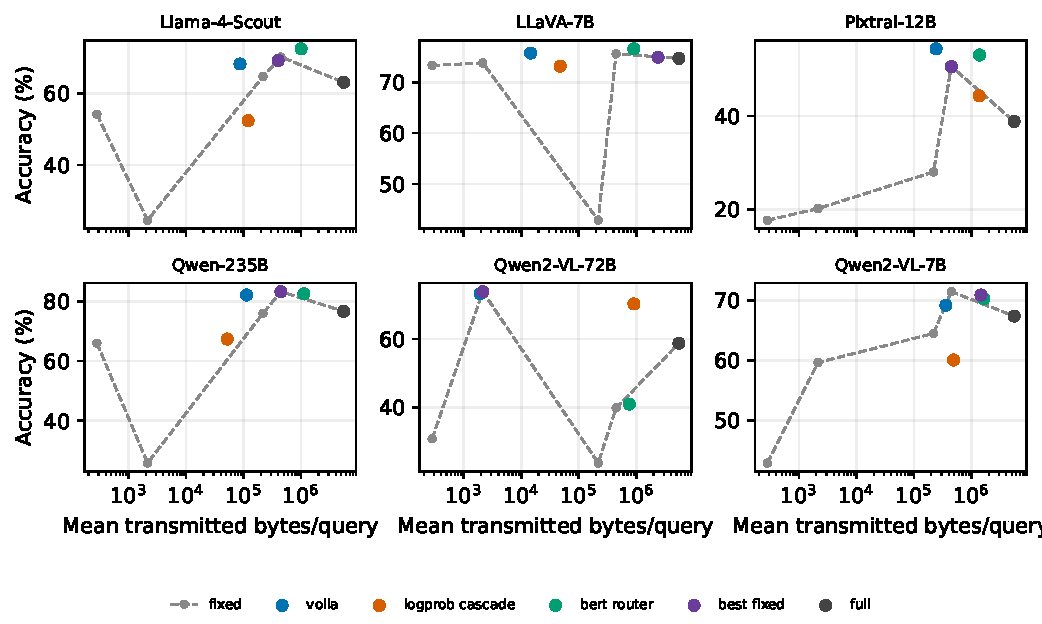
\includegraphics[width=\textwidth]{generated/floodnet_frontier.pdf}
\caption{Measured-byte FloodNet frontier. Every point uses the same
image-grouped test population. Fixed points trace the five cached fidelities;
the cascade includes every representation acquired before stopping.}
\label{fig:frontier}
\end{figure*}

\begin{table*}[t]
\centering
\tableformat
\caption{FloodNet accuracy (\%) and measured MB/query. Best fixed is selected
without the held-out fold; cascade cost is cumulative.}
\label{tab:main}
\resizebox{\textwidth}{!}{\begin{tabular}{lrrrrrrrrrr}
\toprule
Model & Full acc. & MB & Best fixed acc. & MB & Cascade acc. & MB & BERT acc. & MB & VOILA acc. & MB \\
\midrule
Llama-4-Scout & 63.1 & 5.521 & 69.2 & 0.400 & 52.4 & 0.120 & 72.5 & 1.000 & 68.2 & 0.087 \\
LLaVA-7B & 74.7 & 5.521 & 74.9 & 2.386 & 73.1 & 0.047 & 76.5 & 0.903 & 75.7 & 0.015 \\
Pixtral-12B & 38.8 & 5.521 & 50.5 & 0.445 & 44.3 & 1.364 & 53.0 & 1.384 & 54.3 & 0.242 \\
Qwen-235B & 76.6 & 5.521 & 83.2 & 0.445 & 67.3 & 0.052 & 82.5 & 1.120 & 82.1 & 0.113 \\
Qwen2-VL-72B & 58.8 & 5.521 & 73.9 & 0.002 & 70.3 & 0.910 & 40.9 & 0.756 & 73.3 & 0.002 \\
Qwen2-VL-7B & 67.4 & 5.521 & 70.9 & 1.461 & 60.1 & 0.487 & 70.3 & 1.641 & 69.2 & 0.358 \\
\bottomrule
\end{tabular}
}
\end{table*}

\noindent\textbf{Language-conditioned selection occupies a useful but not
universal frontier.} Figure~\ref{fig:frontier} and Table~\ref{tab:main} show
that \system averages \MeanVoilaAccuracy\% at \MeanVoilaMB{} MB/query, compared
with \MeanFullAccuracy\% at \MeanFullMB{} MB for full transmission. It improves
on full-image accuracy by 7.3 points on average because full resolution is not
the VLM accuracy oracle. The advantage is model-dependent: \system is above
best fixed for Pixtral, but best fixed is 0.6--1.7 points higher for four
models. The claim is therefore byte efficiency at a validated accuracy floor,
not universal accuracy dominance.

\noindent\textbf{Measured bytes expose wins hidden by nominal fidelity labels.}
Table~\ref{tab:main} connects each accuracy to the payload actually sent.
Qwen2-VL-72B reaches 73.3\% at roughly 1.9 KB/query; LLaVA reaches 75.7\% at
0.015 MB/query; Pixtral requires 0.242 MB/query for 54.3\%. A policy described
only as choosing ``low,'' ``medium,'' or ``high'' fidelity would miss this
two-order-of-magnitude variation across representations and assets.

\begin{table}[t]
\centering
\tableformat
\caption{Paired \system differences against best fixed (BF) and BERT. Positive
$\Delta$accuracy favors \system; negative $\Delta$MB means fewer bytes.}
\label{tab:paired}
\begin{tabular}{lrrrr}
\toprule
Model & $\Delta$acc BF & $\Delta$MB BF & $\Delta$acc BERT & $\Delta$MB BERT \\
\midrule
Llama-4-Scout & -1.0 & -0.313 & -4.2 & -0.913 \\
LLaVA-7B & +0.8 & -2.372 & -0.8 & -0.888 \\
Pixtral-12B & +3.8 & -0.204 & +1.3 & -1.142 \\
Qwen-235B & -1.1 & -0.333 & -0.4 & -1.008 \\
Qwen2-VL-72B & -0.6 & -0.000 & +32.4 & -0.754 \\
Qwen2-VL-7B & -1.7 & -1.103 & -1.1 & -1.282 \\
\bottomrule
\end{tabular}

\end{table}

\begin{table}[t]
\centering
\tableformat
\caption{Image-clustered 95\% bootstrap intervals for the selected \system
operating point. Bytes are MB/query.}
\label{tab:ci}
\begin{tabular}{lrrrr}
\toprule
Model & Accuracy & 95\% CI & MB & 95\% CI \\
\midrule
Llama-4-Scout & 68.2 & [65.9,70.7] & 0.087 & [0.077,0.096] \\
LLaVA-7B & 75.7 & [73.4,78.0] & 0.015 & [0.011,0.018] \\
Pixtral-12B & 54.3 & [51.8,57.0] & 0.242 & [0.230,0.254] \\
Qwen-235B & 82.1 & [80.2,83.9] & 0.113 & [0.103,0.122] \\
Qwen2-VL-72B & 73.3 & [71.0,75.5] & 0.002 & [0.002,0.002] \\
Qwen2-VL-7B & 69.2 & [66.8,71.6] & 0.358 & [0.336,0.383] \\
\bottomrule
\end{tabular}

\end{table}

\noindent\textbf{Matched comparisons distinguish savings from accuracy
trade-offs.} Table~\ref{tab:paired} uses paired image-clustered resampling.
\system is above the best fixed point for LLaVA and Pixtral and below it by
0.6--1.7 points for four models, while using fewer bytes in every paired
comparison. At matched or higher accuracy it saves up to 2.37 MB/query when
such a fixed point exists. The Qwen2-VL-72B case is a cautionary example for
matched-cost reporting: \system averages 1,916 bytes/query and the fixed
32-pixel tier averages 2,141 bytes/query, producing 73.3\% versus 73.9\%
accuracy at effectively the same transmission cost. Treating only strictly
lower-cost fixed tiers as ``affordable'' would compare against the 281-byte
caption tier and create a spurious 42.6-point gain from a 225-byte gap. BERT is
more accurate on Llama-4 and slightly more accurate on several Qwen/LLaVA
settings, but uses about 0.90--1.64 MB/query on those models. Pixtral is the
clearest adaptive win: 54.3\% at 0.242 MB for \system versus 50.5\% at
0.445 MB for best fixed.

\noindent\textbf{VLM confidence is a weak substitute for pre-retrieval
prediction.} The orange points in Figure~\ref{fig:frontier} show that the
Log-prob Cascade is cheaper than \system for some models but sacrifices
substantial accuracy, including 67.3\% versus 82.1\% on Qwen-235B. On Pixtral
it sends 1.364 MB/query yet reaches only 44.3\%, below \system at both axes.
Because cascade bytes include every attempted fidelity, post-hoc escalation
cannot recover the acquisition cost that pre-retrieval selection avoids.

\noindent\textbf{The effect is stable at the image level even when model gaps
are small.} Table~\ref{tab:ci} reports intervals obtained by resampling images
rather than individual questions. The narrow byte intervals show that the
selected payload mix is not determined by a few unusually large originals.
Accuracy uncertainty is wider for the smaller per-model test folds, which is
why Table~\ref{tab:paired} reports paired differences instead of ranking methods
from point estimates alone.

\subsection{Do byte savings improve timely and mission-level utility?}

\begin{figure}[t]
\centering
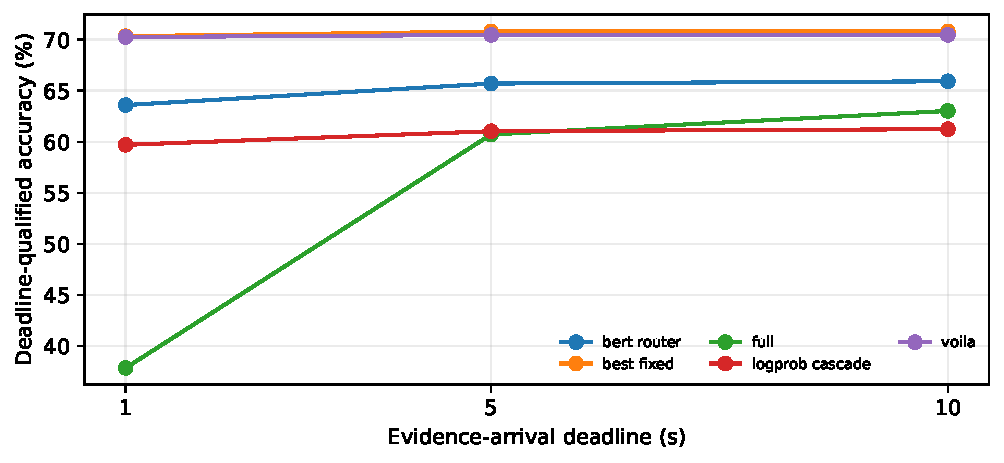
\includegraphics[width=\columnwidth]{generated/deadline_qualified_accuracy.pdf}
\caption{Deadline-qualified accuracy averaged over six recorded cellular
scenarios and six VLMs. A response counts only when it is correct and its
evidence has arrived by the deadline.}
\label{fig:deadline}
\end{figure}

\begin{table*}[t]
\centering
\tableformat
\caption{Recorded-trace one-way uplink serialization results averaged across
models and scenarios. Latencies are seconds; C@1 is one-second completion and
DQA is deadline-qualified accuracy.}
\label{tab:trace}
\begin{tabular}{lrrrrrrrr}
\toprule
Policy & MB & p50 & p95 & C@1 & DQA@1 & DQA@5 & DQA@10 \\
\midrule
Full & 5.521 & 1.428 & 2.959 & 59.3 & 37.9 & 60.7 & 63.0 \\
Best fixed & 0.359 & 0.112 & 0.281 & 99.5 & 70.3 & 70.8 & 70.8 \\
Cascade & 0.497 & 0.034 & 1.237 & 96.3 & 59.7 & 61.0 & 61.2 \\
BERT & 1.134 & 0.054 & 2.370 & 91.7 & 63.6 & 65.7 & 65.9 \\
VOILA & 0.136 & 0.052 & 0.230 & 99.7 & 70.3 & 70.5 & 70.5 \\
\bottomrule
\end{tabular}

\end{table*}

\begin{table}[t]
\centering
\tableformat
\caption{One-second DQA by recorded scenario. BF is best fixed; latency is
\system p95 serialization time in seconds.}
\label{tab:scenario}
\resizebox{\columnwidth}{!}{\begin{tabular}{llrrrr}
\toprule
Carrier & Scenario & Full DQA & BF DQA & VOILA DQA & VOILA p95 \\
\midrule
Tmobile & driving & 32.3 & 70.1 & 69.9 & 0.308 \\
Tmobile & stationary-good & 54.8 & 70.8 & 70.5 & 0.092 \\
Tmobile & weak-signal & 0.0 & 68.7 & 69.8 & 0.674 \\
Verizon & crowded & 22.8 & 70.8 & 70.5 & 0.111 \\
Verizon & stationary-good & 62.8 & 70.8 & 70.5 & 0.079 \\
Verizon & walking & 54.4 & 70.8 & 70.5 & 0.114 \\
\bottomrule
\end{tabular}
}
\end{table}

\noindent\textbf{Byte savings become deadline-qualified answers under short
deadlines.} Figure~\ref{fig:deadline} and Table~\ref{tab:trace} show that
\system reaches \OneSecondVoilaDQA\% DQA at one second, while full-image
transmission reaches \OneSecondFullDQA\%. Its mean p50/p95 serialization
latencies are 0.052/0.230 seconds, compared with 1.428/2.959 seconds for full
images. At five seconds the gap narrows because most full payloads arrive;
this is expected, since routing changes transmission time rather than offline
answer correctness.

\noindent\textbf{A strong fixed policy remains competitive when its payload is
already small.} Table~\ref{tab:trace} shows best fixed at 70.35\% one-second
DQA, about 0.08 point above \system, and 70.81\% at ten seconds, about 0.34
point above. The adaptive benefit appears primarily in bytes and tail latency:
\system reduces mean payload from roughly 0.36--0.37 MB for the compact
baselines to 0.136 MB and reduces p95 serialization to 0.23 seconds. Language
conditioning matters most when the query mix or available fixed point does not
already align with the link.

Thus the headline \MeanByteReduction\% byte reduction and
\OneSecondFullDQA\% to \OneSecondVoilaDQA\% one-second DQA improvement are
relative to full-image transmission. The comparison to best fixed is smaller
and more operationally specific: essentially identical one-second DQA, lower
tail latency, and about a 62\% mean-payload reduction.

\noindent\textbf{The deadline result is not driven by one favorable trace.}
Table~\ref{tab:scenario} separates all six carrier/scenario pairs. Full-image
DQA varies sharply with the recorded opportunity process, whereas \system
remains close to its offline correctness ceiling and keeps p95 serialization
below one second in every aggregated scenario. The table should still be read
as a sensitivity analysis over public cellular traces, not as a carrier or
disaster-network comparison.

\begin{figure}[t]
\centering
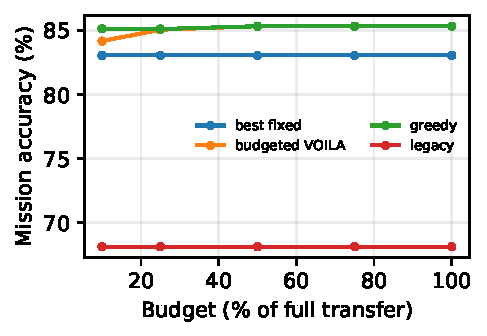
\includegraphics[width=\columnwidth]{generated/mission_accuracy.pdf}
\caption{Qwen-235B mission accuracy for 100-query batches under a shared byte
budget. Budget is expressed as a fraction of sending every original.}
\label{fig:mission}
\end{figure}

\begin{table}[t]
\centering
\tableformat
\caption{Qwen-235B mission accuracy (\%) for batches of 100.}
\label{tab:mission}
\begin{tabular}{lrrr}
\toprule
Policy & 10\% & 25\% & 50\% \\
\midrule
Best fixed & 83.1 & 83.1 & 83.1 \\
Budgeted VOILA & 84.2 & 85.1 & 85.3 \\
Greedy & 85.2 & 85.1 & 85.3 \\
Legacy & 68.1 & 68.1 & 68.1 \\
\bottomrule
\end{tabular}

\end{table}

\noindent\textbf{Batch allocation favors explicit marginal-value sorting.}
Figure~\ref{fig:mission} and Table~\ref{tab:mission} show that budgeted
\system reaches 84.2\% accuracy at 10\% of full-transfer bytes, 1.1 points
above best feasible fixed but 1.0 point below value-per-byte greedy. At 25\%
the adaptive optimizers are effectively tied at 85.1\%, and at 50\% both reach
85.3\%. We therefore do not present the calibrated per-query policy as the best
batch allocator. When a whole batch and a hard shared budget are known in
advance, sorting predicted marginal gains per byte is preferable; the per-query
VOI rule is the online policy for independent arrivals or unknown future demand.
The cached oracle reaches 90.5\% at the 10\% budget, leaving meaningful
headroom in predicted marginal value.

\subsection{What enables the gain, and where does it fail?}

\begin{table}[t]
\centering
\tableformat
\caption{Calibration, feature, and template-holdout stress results. Main and
template columns are accuracy (\%); ``Struct only'' removes TF--IDF. The final
column is the validation-recommended calibrator.}
\label{tab:robustness}
\resizebox{\columnwidth}{!}{\begin{tabular}{lrrrrl}
\toprule
Model & Main & Template & $\Delta$ & Struct only & Cal. \\
\midrule
Llama-4-Scout & 68.2 & 45.7 & -22.6 & 68.4 & iso \\
LLaVA-7B & 75.7 & 58.3 & -17.4 & 76.1 & shared\_platt \\
Pixtral-12B & 54.3 & 26.2 & -28.1 & 53.8 & none \\
Qwen-235B & 82.1 & 45.0 & -37.1 & 81.1 & none \\
Qwen2-VL-72B & 73.3 & 44.2 & -29.1 & 73.4 & iso \\
Qwen2-VL-7B & 69.2 & 48.8 & -20.4 & 68.7 & none \\
\bottomrule
\end{tabular}
}
\end{table}

\begin{table}[t]
\centering
\tableformat
\caption{Calibration ablation as accuracy (\%)/MB per query. Each variant uses
the same split and validation-only operating-point rule.}
\label{tab:calibration}
\resizebox{\columnwidth}{!}{\begin{tabular}{lrrr}
\toprule
Model & None & Independent iso & Shared Platt \\
\midrule
Llama-4-Scout & 67.8/0.076 & 68.2/0.086 & 69.5/0.124 \\
LLaVA-7B & 75.8/0.001 & 75.7/0.015 & 75.8/0.002 \\
Pixtral-12B & 54.8/0.224 & 54.3/0.232 & 54.0/0.230 \\
Qwen-235B & 83.2/0.134 & 82.1/0.118 & 81.2/0.118 \\
Qwen2-VL-72B & 74.0/0.002 & 73.3/0.002 & 74.0/0.002 \\
Qwen2-VL-7B & 69.3/0.356 & 69.2/0.354 & 69.3/0.472 \\
\bottomrule
\end{tabular}
}
\end{table}

\noindent\textbf{Calibration makes the utility comparable, but isotonic is not
uniformly the most accurate variant.} Tables~\ref{tab:calibration}
and~\ref{tab:robustness} report the outcomes and the calibrator recommended on
held-out validation data. Independent isotonic is the
primary definition because Eq.~\ref{eq:utility} requires per-fidelity
probabilities and it avoids sharing one scale across heterogeneous
representations. In the ablation, however, no calibration is slightly better
for Pixtral, Qwen-235B, Qwen-72B, and Qwen-7B in the selected operating point,
while validation recommends shared Platt for LLaVA and independent isotonic for
Llama-4 and Qwen-72B. The theory motivates calibrated probabilities for the
utility calculation; the finite-sample result is weaker and more useful:
calibration is a model-selection choice, not a guaranteed accuracy improvement.
The main empirical failure of uncalibrated confidence is the VLM Log-prob
Cascade in Figure~\ref{fig:frontier}, not a claim that isotonic wins every
aggregate routing metric.

\begin{table}[t]
\centering
\tableformat
\caption{Linguistic feature ablation as accuracy (\%)/MB per query. Structural
features exclude TF--IDF; type-only retains only broad question form.}
\label{tab:features}
\resizebox{\columnwidth}{!}{\begin{tabular}{lrrr}
\toprule
Model & TF--IDF+struct & Struct only & Type only \\
\midrule
Llama-4-Scout & 68.2/0.086 & 68.4/0.089 & 69.0/0.790 \\
LLaVA-7B & 75.7/0.015 & 76.1/0.001 & 74.5/0.233 \\
Pixtral-12B & 54.3/0.232 & 53.8/0.229 & 49.5/0.289 \\
Qwen-235B & 82.1/0.118 & 81.1/0.110 & 85.3/0.298 \\
Qwen2-VL-72B & 73.3/0.002 & 73.4/0.003 & 73.7/0.002 \\
Qwen2-VL-7B & 69.2/0.354 & 68.7/0.302 & 70.7/0.761 \\
\bottomrule
\end{tabular}
}
\end{table}

\noindent\textbf{Simple linguistic structure carries much of the signal.}
Table~\ref{tab:features} shows that structural features remain close to the
full feature set for several models, and question-type-only features improve
Qwen-235B to 85.3\%, but at 0.298 MB/query versus 0.118 MB/query for the full
feature set. TF--IDF helps distinguish templates within a broad class and often
improves the cost side of the trade-off, but its gains are corpus-dependent.
This supports the motivating hypothesis that language is practically useful
while rejecting the stronger claim that surface form fully determines fidelity.

\noindent\textbf{Unseen language is the dominant failure mode.}
Table~\ref{tab:robustness} shows that holding out entire question templates
reduces accuracy for every model by 17.4--37.1 points; Qwen-235B falls from
82.1\% to 45.0\%. Image-grouped folds prevent visual leakage, but they do not
by themselves establish robustness to new ways of asking. A deployment needs
template-diverse calibration data, shift detection, and a conservative
fallback when the question is outside the training language.

\noindent\textbf{The router is small enough to remain outside the remote
inference path.} The saved Qwen-235B artifact has a 4.12 ms warm median and
5.32 ms p95 on the reference CPU, occupies 234,666 bytes, and peaks at 162 MB
process memory. Figure~\ref{fig:system} therefore reflects a practical
placement: selection can occur where the query and metadata are available,
without invoking a visual encoder before acquisition.

\subsection{Failure analysis}

\begin{figure}[t]
\centering
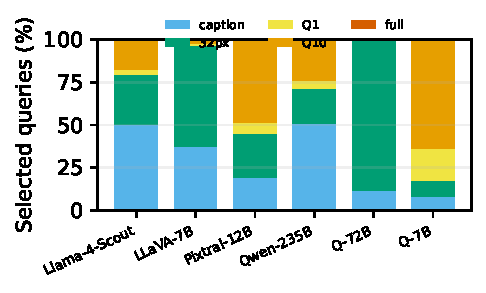
\includegraphics[width=\columnwidth]{generated/selection_distribution.pdf}
\caption{Test-time \system selections by target VLM. Language is shared, but
the learned fidelity mixture changes with the VLM's measured behavior.}
\label{fig:selection}
\end{figure}

\begin{table}[t]
\centering
\tableformat
\caption{Failure decomposition (\%). Oracle is the fraction answerable by at
least one fidelity; Exact selects its cheapest successful tier; Under selects
an incorrect tier despite an available answer; Over answers correctly with
more bytes than the cached oracle; None is unanswerable at all five tiers.}
\label{tab:failure}
\resizebox{\columnwidth}{!}{\begin{tabular}{lrrrrr}
\toprule
Model & Oracle & Exact & Under & Over & None \\
\midrule
Llama-4-Scout & 88.6 & 51.8 & 20.3 & 16.4 & 11.4 \\
LLaVA-7B & 83.7 & 33.6 & 8.0 & 42.1 & 16.3 \\
Pixtral-12B & 79.4 & 40.9 & 25.1 & 13.4 & 20.6 \\
Qwen-235B & 90.2 & 59.4 & 8.2 & 22.7 & 9.8 \\
Qwen2-VL-72B & 86.3 & 46.2 & 13.0 & 27.1 & 13.7 \\
Qwen2-VL-7B & 84.2 & 7.8 & 14.9 & 61.4 & 15.8 \\
\bottomrule
\end{tabular}
}
\end{table}

\noindent\textbf{The selected representation depends on the target model, not
only the wording.} Figure~\ref{fig:selection} shows markedly different fidelity
mixtures although every model sees the same question population. Qwen-72B is
served mainly by the 32-pixel representation, whereas Pixtral and Qwen-7B
require a broader mix of compressed images. Thus the linguistic signal predicts
model-specific success; it is not a universal mapping from question type to
resolution.

\noindent\textbf{The Qwen2-VL-72B full-resolution drop should be treated as a
model/preprocessing interaction, not as evidence that information hurts.}
Table~\ref{tab:fixed} shows Qwen2-VL-72B at 73.9\% on 32-pixel inputs but
58.8\% on full images, a 15.1-point reversal. The error is concentrated in the
FloodNet condition-recognition mix where compressed inputs already preserve the
coarse scene label. A plausible mechanism is Qwen2-VL's dynamic image
preprocessing on large aerial originals: full-resolution files change tiling,
token allocation, and prompt packing relative to the tiny PNG, and may expose
texture that is irrelevant to the answer-matching label. We therefore report
the anomaly explicitly and avoid using it as a causal claim; resolving it
requires model-internal preprocessing traces or a manual answer audit.

\noindent\textbf{Under-acquisition is the consequential reducible error.}
Table~\ref{tab:failure} distinguishes cheap mistakes from expensive successes.
An under-acquired query is wrong even though at least one cached fidelity could
answer it; better probability estimation could recover that accuracy. An
over-acquired query is correct but spends more bytes than the hindsight oracle;
better cost ranking could recover efficiency. The remaining ``None'' cases
cannot be repaired by fidelity routing because the cached VLM fails at every
representation.

\noindent\textbf{The oracle gap is not one problem.}
Table~\ref{tab:failure} shows that exact oracle selection is a minority outcome
for several models, yet aggregate accuracy can remain high because different
fidelities often answer the same query correctly. Closing the gap therefore
requires two distinct interventions: richer language or weak visual metadata
to reduce under-acquisition, and sharper calibrated cost differences to reduce
over-acquisition. A more complex router that addresses only one may move the
wrong axis of Figure~\ref{fig:frontier}.

\begin{table}[t]
\centering
\tableformat
\caption{Secondary external-validity evidence from a cached multi-dataset
study. Cost is its normalized acquisition proxy,
not measured FloodNet bytes, so it is not pooled with the primary results.}
\label{tab:external}
\begin{tabular}{lrrr}
\toprule
Dataset & Models & Accuracy & Normalized cost reduction \\
\midrule
VQAV2 & 6 & 72.8 & 34.8\% \\
GQA & 6 & 68.1 & 36.6\% \\
TEXTVQA & 6 & 89.0 & 55.6\% \\
\bottomrule
\end{tabular}

\end{table}

\noindent\textbf{The linguistic signal is not unique to flood questions.}
Table~\ref{tab:external} retains a compact VQA-v2, GQA, and TextVQA check from
the broader cached study~\cite{goyal2017vqav2,hudson2019gqa,singh2019textvqa}.
It is secondary evidence because its cost model differs from the measured-byte
FloodNet protocol. The consistent savings motivate broader evaluation, but do
not substitute for same-protocol replication on additional domains.

\section{Discussion}
\label{sec:discussion}

\textbf{Pre-retrieval selection is an information decision, not a compression
codec.} A codec maps an image to fewer bits after the image is available.
\system instead chooses among representations that already exist at a storage
or network boundary. The distinction explains why byte metadata is legitimate
input while pixels are not: metadata is part of the index used to decide what
to fetch. The policy can select a caption, thumbnail, compressed image, or
original without decoding all alternatives.

\textbf{The method is complementary to model routing.} After \system acquires
one representation, RouteLLM-style logic may still choose a remote model, and
an early-exit mechanism may still shorten its computation. Conversely, a model
router cannot retroactively remove bytes already retrieved. A joint policy
would optimize a pair $(f,m)$ over fidelity and model, but would require
calibrated success estimates for every pair and substantially more offline
labels.

\textbf{The 95\% rule is a deployment contract rather than a universal
objective.} We use it to prevent the byte penalty from selecting a cheap but
unacceptably inaccurate point. A medical archive may demand a higher floor; a
best-effort search interface may accept a lower one. Equation~\ref{eq:utility}
supports either choice, but the operating point must be selected without test
data and reported with the corresponding failure cost.

\textbf{Fallbacks should respond to linguistic uncertainty.} The
template-holdout experiment suggests a practical safeguard: route questions
far from the calibration language to a conservative fidelity rather than
trusting an extrapolated probability. Conformal abstention, nearest-template
distance, or a small online calibration buffer could implement this behavior.
The current experiments quantify the need for such a mechanism but do not
evaluate one.

\section{Related Work}
\label{sec:related}

\textbf{Visual question answering and linguistic difficulty.}
VQA established free-form language queries over images~\cite{antol2015vqa};
VQA-v2, GQA, and TextVQA expose complementary language priors, compositional
reasoning, and OCR requirements~\cite{goyal2017vqav2,hudson2019gqa,
singh2019textvqa}. Analyses consistently find question type predictive of
difficulty and failure~\cite{kafle2017analysis,agrawal2018dont}. \system uses
that regularity for a different decision: estimating the information needed
before acquiring the visual input.

\textbf{Pre-retrieval prediction and multimodal retrieval.}
Pre-retrieval query-performance prediction estimates retrieval difficulty from
lexical and syntactic features without executing retrieval~\cite{
zhao2008predicting,hauff2008improved,mothe2005linguistic}. RAG and multimodal
RAG retrieve external text or images before generation~\cite{lewis2020rag,
yasunaga2023retrievalaugmented,chen2022murag}. These systems typically choose
which item to retrieve at a fixed representation quality. \system extends the
pre-retrieval view to choosing the fidelity of an already identified visual
asset.

\textbf{Adaptive inference and routing.}
FrugalGPT, RouteLLM, hybrid routing, and related routers choose among model
tiers after the input is available~\cite{chen2023frugalgpt,wang2024routellm,
ding2024hybrid,shnitzer2023large}. Early-exit methods shorten computation when
intermediate confidence is sufficient~\cite{zhou2020bert,elbayad2020depth,
schuster2022confident}. These methods optimize how a retrieved input is
processed. Pre-retrieval fidelity selection instead optimizes what input is
acquired, and can precede any of them.

\textbf{Adaptive visual fidelity.}
Learned image compression, bandwidth-adaptive video analytics, and edge
offloading reduce representation, sampling, or compute after a stream or model
stage is available~\cite{toderici2016variablerateimagecompression,
jiang2018chameleon,du2020dds,li2020reducto,kang2017neurosurgeon,
chu2024mobilevlm,farazi2021accuracy,weng2024learning}. Semantic communication
similarly transmits task-relevant meaning rather than raw bits, but typically
learns an encoder over the observed signal~\cite{xie2021semantic}. Recent
multimodal work adapts visual token budgets or resolution inside the VLM, as in
Matryoshka multimodal models and FastV-style pruning~\cite{
cai2024matryoshka,chen2024fastv}. CARES selects resolution using a compact VLM
over the image, and prompt-guided prefiltering identifies relevant regions after
image access~\cite{kimhi2025cares,azizian2026promptguided}. \system targets the
stricter boundary at which pixels are not yet available: it chooses which
cached representation should be acquired at all. Tiered mobile and cloud storage
further motivates treating acquisition as a first class cost~\cite{
lonn2019smartphonepictureorganizationhierarchical,aws_s3_storage_classes,
hort2021survey}.

\textbf{Value of information and active acquisition.}
Value-of-information methods choose whether the expected benefit of evidence
justifies its cost~\cite{bilgic2011value}. Cost-sensitive feature acquisition
and active multimodal acquisition apply related principles to tabular or
sequential observations~\cite{karkkainen2019cost,kossen2022active}. \system
specializes this decision to mutually available image representations, using
language-conditioned VLM correctness as value and measured payload bytes as
cost.

\section{Limitations}
\label{sec:limitations}

\textbf{Language does not uniquely determine visual need.}
The template-holdout losses are large, and visually ambiguous questions can
require different fidelity despite identical wording. The current policy has
no access to scene content before selection and therefore cannot resolve such
cases.

\textbf{Cached representations define the accounting boundary.}
Captions and VLM answers are reused from prior runs. Caption creation latency
and energy are excluded because captions are generated once during ingestion.
This assumption is appropriate for repeatedly queried archives, but not for a
one-shot stream with no preprocessing. Correctness also inherits the cached
answer-matching procedure and service version.

\textbf{The network experiment is a serialization simulation.}
CellReplay traces are public 5G proxies rather than disaster deployments. We
model recorded delivery opportunities, delay offsets, packetization, and
circular start phases, but omit TCP state, protocol headers, retransmission
semantics, radio energy, downlink, VLM latency, and human response. The reported
DQA is consequently not an end-to-end operational latency claim.

\textbf{One dataset anchors the measured-byte claim.}
The primary protocol is FloodNet-centered because it provides the complete
common population across six cached VLMs. The secondary datasets use an older
normalized cost model. Same-protocol measured-byte replication is needed
before generalizing effect sizes to document, medical, or consumer-photo
retrieval.

\section{Conclusion}

The fidelity of visual evidence is an acquisition decision, not merely a VLM
preprocessing parameter. \system shows that question language can guide this
decision before retrieval or transmission: calibrated, fidelity-specific
success estimates identify a useful accuracy--byte frontier without accessing
pixels or invoking the remote model. On the measured FloodNet population this
removes \MeanByteReduction\% of full-image bytes on average and turns the
savings into substantially more correct answers by a one-second upload
deadline. The fixed-policy and template-shift results also define the boundary
of the contribution. Language is a strong prior over information need, not a
complete substitute for visual context. More broadly, the work argues that a
multimodal system should estimate the value of evidence before paying to
acquire it.

\clearpage
\begingroup
\let\footnotesize\scriptsize
\bibliographystyle{IEEEtran}
\bibliography{example_paper}
\endgroup

\end{document}
